\chapter{ODS Output for Website Integration}
\index{Website Integration}
\index{Website Templates}
Many web sites have a framework that web pages must fit into 
before they will be published.  Usually this means
editing the html pages and pasting in some chunk of HTML from
some files the website authors have provided.
Usually there is one file to replace the top section of the
web page and another to replace the bottom.  
The tagsets in this chapter will create HTML that
is ready for integration with any website.  

\section{The Problem}
Most websites want webpages to be enclosed with some sort of
image and navigation menu at the top and/or bottom.  Most of this
is usually enclosed in some sort of table to control the layout.

This enclosing HTML is usually put in two files so that it is easy
to include them as the top and bottom of each web page.  Prior to
SAS 9.1 there were two ways to do this.  The hardest way is to use
the no\_top and no\_bot options along with some datastep to write
the file templates.  Starting with SAS 8.2 it became possible to
create a tagset that included the text from the website's framework
files.  This is really the simplest way to do this, but it leads
to dual maintenance because everytime the files change, the tagset
needs to have the same changes.

\index{Website Integration}
\index{Website Templates}
\index{Statements!Putl}
\index{Putl}
If that is the route you wish to take there is a put command that
will help.  'Putl' is just like put except that it has an automatic
newline at the end.  That means you can copy and paste in a block
of text and place a putl ' at the beginning and a '; at the end of
each line.  That's not too hard but can be painful if the framework
files change very often.

The framework files usually include everything that goes in an HTML
document down to and including the body tags.  All of your content
goes inbetween with no need to define the basic HTML document.  At
the very least the solution needs to eliminate the output from the
events above the start and below the finish of the doc\_body event.

The most difficult part of this is that somehow, the stylesheet for
the ODS output will have to be incorporated into the middle of the
framework text.  If your web designers are nice, they may be willing
to place an ods generated stylesheet with their other stylesheets.
They may even put a reference to it in their framework file.  In
that case the tagset will be easy.  Either way, a working tagset
can be created.

\section{Alternate Behavior for existing options}
The first step towards this solution is to eliminate all the events
above and below the body tags.  ODS already gives options to do
that.  All that is needed is to detect when those options are set.
Then detect if there are files that can be used in place of the
head and foot sections of the document.

\index{Options!No\_Top\_Matter}
\index{Options!No\_Bottom\_Matter}
\index{Options!No\_Top}
\index{Options!No\_Bot}
\index{Variables!No\_Top}
\index{Variables!No\_Bot}
Macro variables, or alias can be used to specify the files to read.
If both the no\_top\_matter and no\_bottom\_matter options are used
with file name specifications, then the tagset can behave as desired.
Otherwise normal behavior will be the way to go.

\subsection{Explore}
Running an event map with the notop and nobot options shows that there are variables in
the tagset called no\_top and no\_bot that indicate these options were set.  That will
be very useful.

\index{Events!Initialize}
The trick to this tagset is using the initialize event to advantage.  The initialize
event always happens.  But when no\_top and no\_bot is used the first and last events
are somewhat variable.   The first event could be system\_titles, or not.  The last could
be system\_footers, or not.  Reviewing the available events shows that no\_bot causes
the end to be unpredictable.  Luckily there are not that many events in the bottom
section of an html document.  As usual, the initialize event can be used to set things up, and
redefine the events in the bottom section to do the right thing.  That means that
all the external controls need is the no\_top option with some method of passing two 
filenames to read.

\section{Reading an external file}

\index{Functions!filename}
\index{Functions!fopen}
\index{Functions!fread}
\index{Functions!fget}
\index{Functions!Return Code}
\index{Statements!Eval}
\index{Statements!Set}
\index{DataStep!Functions}
The key to this tagset is reading an external file.  That example is shown
on page \pageref{readfile}.  This example will build on that functionality.

Your website's authors will probably have two files that may resemble the following
HTML code.  The top section defines the html document and starts the body section
of the page and creates some tables for layout.  There is a table along the top for
the Company logo and navigation.  Below that is another table with one row and three
cells.  The first cell contains another table with more navigation menus.  the second
cell is where The sas output will go.  The second file closes everything up, puts a
table across the bottom for more navigation, contacts, copyright notices and the like.

\begin{Verbatim}[frame=lines, framesep=3mm, label={Sample}]

<!DOCTYPE html PUBLIC "-//W3C//DTD XHTML 1.0 Transitional//EN"
    "http://www.w3.org/TR/xhtml1/DTD/xhtml1-transitional.dtd">

<html xmlns="http://www.w3.org/1999/xhtml">
  <head>
    <meta name="generator" content="HTML Tidy, see www.w3.org" />
    <meta content="text/html; charset=iso-8859-1"
    http-equiv="Content-Type" />

    <title>Your website name</title>
    <meta name="description" content="Your website name" />
    <meta name="keywords" content="SAS, ODS, Markup, HTML, XML" />

    <link rel="shortcut icon" href="/favicon.ico" type="image/x-icon" />
    <link rel="icon" href="/fav_icon.ico" type="image/x-icon" />
    <style type="text/css">
    <!--
    .main{Background-color:#E0E0E0;
          color:#000000;
         }

    a:link { color:#0066AA }
    a:visited { color:#004488 }
    a:active { color:#004488 }

    .layout_table{cellspacing: 0;
                  padding: 0;
                  borderwidth: 0px;
                  width: 100%;
         }
    .nav_table{cellspacing: 0;
                  borderwidth: 0px;
                  width: 50px;
                  background-color: #00DD55;
         }
    .nav_label{color: #000088;
               font-size: medium;
               font-weight: bold;
         }
    .output_cell{color: #E0E0E0;
         }
    </style>
  </head>

  <body class="main">

    <!-- Beginning of Top headline and navigation table -->
    <table class="layout_table">
      <tr>
        <td><a href="http://www.yourdomain.org/index.html">
        <img src="gifs/logo.gif" height="94" width="306"
        alt="Logo Image alt text: Your Company: Slogan" border="0" /></a>
        </td>

        <td align="right" valign="bottom">

          <form action="http://www.yourdomain.org/cgi/region.cgi"
          method="get">
            <br />
            <span class="nav_label">Select your Region:</span>
            <br />
            <select name="goto">
              <option value="http://www.yourdomain.org/region1"> Region 1 </option>

              <option value="http://www.yourdomain.org/region2">
                Region 2
              </option>

              <option value="http://www.yourdomain.org/region3">
                Region 3
              </option>

              <option value="http://www.yourdomain.org/region4">
                Region 4
              </option>

              <option value="http://www.yourdomain.org/region5">
                Region 5
              </option>

              <option value="http://www.yourdomain.org/region6">
                Region 6
              </option>
            </select><input type="submit" value=" Go " /><br />

          </form>
        </td>
      </tr>
    </table>
    <hr size="1" noshade="noshade" />

    <!-- Beginning of main table -->
    <table class="layout_table">
      <tr>

        <!-- Beginning of Left Side Navigation Bar. -->
        <td valign="top">
          <table class="layout_table">
            <tr>
              <td>
                <table class="nav_table">
                  <tr>
                    <td>
                      <p><font class="nav_label"><b>News</b></font>
                      <small><br />

                       <a href="news/newsflash.html">Announcements</a><br />

                       <a href="news/press.html">In the Press</a><br />
                       <a href="news/index.html">More ...</a>
                       </small></p>

                      <p><font class="nav_label"><b>Company</b></font>
                      <small><br />

                       <a href="./contact/index.html">Contact Information</a><br />
                       <a href="./about/index.html">About</a><br />
                      </small></p>

                      <form action="http://www.yourdomain.org/cgi/search.cgi"
                       method="get">

                        <small>Search for:<br />
                        <input type="text" name="words" size="10" />
                        <input type="hidden" name="max" value="25" />
                        <input type="hidden" name="source" value="www" />
                        <input type="submit" value="Go" />
                        </small>
                      </form>
                    </td>
                  </tr>
                </table>
              </td>
            </tr>

          </table>
        </td>
        <!-- End of Left Side Navigation Bar. -->

        <!-- Beginning of Center - Output Panel -->
        <td class="output_cell">
\end{Verbatim}

The ending of your website's pages may look something like this

\begin{Verbatim}[frame=lines, framesep=3mm, label={Sample2}]
        </td>
        <!-- End of Center - OutputPanel -->

        <!-- beginning of Right - Navigation Panel -->
        <td align="right">
           <table class="nav_table" >
             <tr><td>
               <ul>
                 <li> More Navigation:</li>
                 <ul>
                   <li> Navigation1</li>
                   <li> Navigation2</li>
                 </ul>
               </ul>
             </td></tr>
           </table>
        </td>
        </tr>
    <!-- End of Middle - Layout table -->
   </table>

   <table class="layout_table" >
   <tr>
   <td align="center">
    <hr size="1" noshade="noshade" /><br/>
       Copyright 2004 Your Company name. 
   </td>
   </tr>
   </table>

</body>
</html>
\end{Verbatim}

\section{The Solution}
The following tagset will read the files given through the tagset alias or 
a macro variable called infiles.  Alias or infiles should be two
filenames separated by a space.   
If tagset alias is set to 'default' then the 
set\_default\_files event is used to set the default file names.
By using a separate event, this tagset can be used as a parent
tagset, where only the set\_default\_files event is redefined.
This also allows normal no\_top behavior if no files are specified.  

Another key to this tagset is that only external stylesheets are
allowed.  It is possible to make embedded stylesheets work.  But
that behavior is not really desirable in this case because our network
administrators wouldn't like embedded stylesheets in our files.  
A stylesheet file must be specified on the ods statement when using
this tagset.

\subsection{Initialization Timing}
\index{Tagsets!short\_map}
\index{Events!Proc}
\index{Events!Initialize}
\index{Events!Initialize!Timing}
\index{Files!Stylesheet}
\index{Variables!No\_Top}
Upon trying this method with the stylesheet option, it can be seen that the initialize event
doesn't work quite right.  That's because initialize happens once.  At the very beginning.
The stylesheet file is created before the body file, so that's when it happens.  No\_top isn't
set for the stylesheet, so the head section of the body file is never printed.  
The solution can be found
by running the same output through the short\_map tagset - with the same ods statement options.
What can be seen is that the proc event always comes out the first thing.  Using the first
proc event to print the top of the file template will work just fine.
 
The best solution is for the website's templates include an ods stylesheet. 
In that case specifying a stylesheet on the ods statement won't be 
necessary.  That would also insure that all ODS output always matches
the website.  All things considered this is still a fairly simple tagset.  The
most complex parts are the things that make it work invisibly for users
who don't want or need this special behavior.

\begin{fvcode}{Web_integration}{Website integration Tagset}
/*----------------------------------------------------------------*/
/*-- Reading a file in using datastep functions.  This example  --*/
/*-- comes straight out of the online documentation             --*/
/*-- for fread().                                               --*/
/*----------------------------------------------------------------*/
proc template;
    define tagset tagsets.website;
        parent=tagsets.html4;
        embedded_stylesheet=no;

        define event initialize;

            do /if $options;
               do /if $options['HEAD_FILE']; 
                   set $head_file $options['HEAD_FILE'];
               done;
               do /if $options['FOOT_FILE']; 
                   set $foot_file $options['HEAD_FILE'];
               done;
               do /if cmp($options['DEFAULT_FILES'], 'yes'); 
                    set $head_file 'default_head.html' /if ^$head_file;
                    set $foot_file 'default_foot.html' /if ^$head_file;
               done;
            done;

            putlog "Infiles are" " :" $head_file "  " $foot_file;

            set $filename $head_file;

            /*--------------------------------------------eric-*/
            /*-- Set a flag so the ending document tags      --*/
            /*-- can be suppressed.                          --*/
            /*-----------------------------------------8Nov 03-*/
            do /if $infiles);
                set $read_files 'true';
                set $filrf "headfile";
                set $read_head "true";
            done;
        end;

        define event proc;
            start:
                do /if no_top;
                    do /if $read_head;
                        trigger readfile;
                        unset $read_head;
                    done;
                done;
        end;


        define event head_search;
            trigger integrated_link /if contains($file_record, '</head>');
        end;

        define event integrated_link;
            put '<style type="text/css">' CR '<!--' CR;
            trigger alignstyle;
            put '-->' CR '</style>' CR ;
        
            set $urlList stylesheet_url;
            set $urlList stylesheet_name /if !$urlList;
            trigger urlLoop ;
            unset $urlList;
        end;

        define event readfile;
            
            /*------------------------------------------------*/
            /*-- Set up the file and open it.               --*/
            /*------------------------------------------------*/
            putlog "Reading in file: " $filename;

            eval $fid 0;
            
            eval $rc filename($filrf, $filename);
            
            eval $fid fopen($filrf);
            do /if missing($fid);
                putlog "Error: Could not open file, " $filename;
                break;
            done;


            /*---------------------------------------------------*/
            /*-- datastep functions  will bind directly to the --*/
            /*-- variable space as it exists.                  --*/
            /*--                                               --*/
            /*-- Tagset variables are not like datastep        --*/
            /*-- variables but we can create a big one full    --*/
            /*-- of spaces and let the functions write to it.  --*/
            /*--                                               --*/
            /*-- This creates a variable that is 200 spaces so --*/
            /*-- that the function can write directly to the   --*/
            /*-- memory location held by the variable.         --*/
            /*-- in VI, 200i<space>                            --*/
            /*---------------------------------------------------*/
            set $file_record  "

                                  ";

            /*-------------------------------------------------*/
            /*-- Loop over the records in the file           --*/
            /*-------------------------------------------------*/
            do /if $fid > 0 ;

                do /while fread($fid) = 0;

                    set $rc fget($fid,$file_record ,200);

                    trigger head_search;
                    
                    /* trimn to get rid of the spaces at the end. */
                    put trimn($file_record ) nl;

                done;
            done;

           /*----------------------------------------------------*/
           /*-- close up the file.  set works fine for this.   --*/
           /*----------------------------------------------------*/

            set $rc close($fid);
            set $rc filename($filrf);

        end;

        define event doc;
            start:
                set $doctype '<!DOCTYPE html PUBLIC "-//W3C//DTD HTML 4.01 Transitional//EN">';
                set $framedoctype '<!DOCTYPE html PUBLIC "-//W3C//DTD HTML 4.01 Frameset//EN">';
                put $doctype CR;
                put "<html>" CR;

            finish:
                do /if $read_files;
                    set $filename scan($infiles, 2, ' ');
                    set $filrf "footfile";
                    trigger readfile;
                    break;
                done;

                put "</html>" CR;
        end;

        define event doc_body;
            put '<body onload="startup()"';
            put ' onunload="shutdown()"';
            put  ' bgproperties="fixed"' / WATERMARK;
            putq " background=" BACKGROUNDIMAGE;
               trigger style_inline;
            put ">" CR;
            trigger pre_post;
            put          CR;
            trigger ie_check;

          finish:
            trigger pre_post;

            break /if $read_files;
            put "</body>" CR;
        end;

end;

run;


ods tagsets.shortmap stylesheet="stylesheet.map" 
                          file="website.map"(notop) ;

ods tagsets.website stylesheet="website.css" 
                          file="website.html"(notop) 
                         options(default_files = 'yes');

proc print data=sashelp.class; run;
    
ods tagsets.website close;
ods _all_ close;
\end{fvcode}

\section{Summary}
\index{Website Integration}
The output using these particular template files is shown 
in figure \vref{website_out}.  
Working with the authors of your website should enable you to create some very
nice looking output.  All of which is immediately ready for integration.
        
\begin{goutput}{startpage2_out}{Website integration}
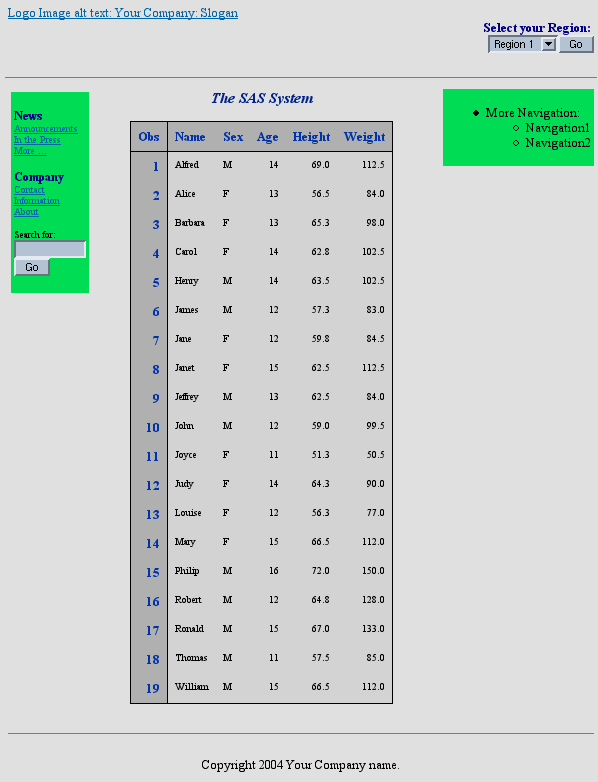
\includegraphics[width=6in]{website.png}
\end{goutput}
